Determine if the following are convex functions
\begin{enumerate}[label=\thechapter.\arabic*,ref=\thechapter.\theenumi]
\numberwithin{equation}{enumi}
\numberwithin{figure}{enumi}
\numberwithin{table}{enumi}
\item
	\begin{enumerate}
\item Detrmine whether the function $f\brak{x} = \brak{2x-1}^2 + 3$ is convex or not. \\ 
\solution 
\label{12/6/5/1/1/conv}
\iffalse 
\documentclass[12pt]{article}
\usepackage{graphicx}
\usepackage[none]{hyphenat}
\usepackage{graphicx}
\usepackage{listings}
\usepackage[english]{babel}
\usepackage{graphicx}
\usepackage{caption} 
\usepackage{booktabs}
\usepackage{array}
\usepackage{amssymb} % for \because
\usepackage{amsmath}   % for having text in math mode
\usepackage{extarrows} % for Row operations arrows
\usepackage{listings}
\lstset{
  frame=single,
  breaklines=true
}
\usepackage{hyperref}
\usepackage{mathtools}

%Following 2 lines were added to remove the blank page at the beginning
\usepackage{atbegshi}% http://ctan.org/pkg/atbegshi
\AtBeginDocument{\AtBeginShipoutNext{\AtBeginShipoutDiscard}}


%New macro definitions
\newcommand{\mydet}[1]{\ensuremath{\begin{vmatrix}#1\end{vmatrix}}}
\providecommand{\brak}[1]{\ensuremath{\left(#1\right)}}
\providecommand{\sbrak}[1]{\ensuremath{{}\left[#1\right]}}
\providecommand{\norm}[1]{\left\lVert#1\right\rVert}
\providecommand{\abs}[1]{\left\vert#1\right\vert}
\newcommand{\solution}{\noindent \textbf{Solution: }}
\newcommand{\myvec}[1]{\ensuremath{\begin{pmatrix}#1\end{pmatrix}}}
\let\vec\mathbf


\begin{document}

\begin{center}
\title{\textbf{Convex Optimization}}
\date{\vspace{-5ex}} %Not to print date automatically
\maketitle
\end{center}
\setcounter{page}{1}

\section{12$^{th}$ Maths - Chapter 6}
This is Problem-1(i) from Exercise 6.5
\begin{enumerate}
		\fi
The given function is 
\begin{align}
        \label{eq:/12/6/5/1/1/convEq5}
	f\brak{x} &= \brak{2x-1}^2 + 3 \\ 
	&= 4x^2+4x+4 \\
	\therefore a &= 4, > 0
\end{align}
Hence, the function in equation \eqref{eq:/12/6/5/1/1/convEq5} is convex
	from \ref{prop:app/convconvconvex_def}.
%
The figure is as shown in Fig\ref{fig:/12/6/5/1/1/convFig1}
\begin{figure}[!h]
	\begin{center}
		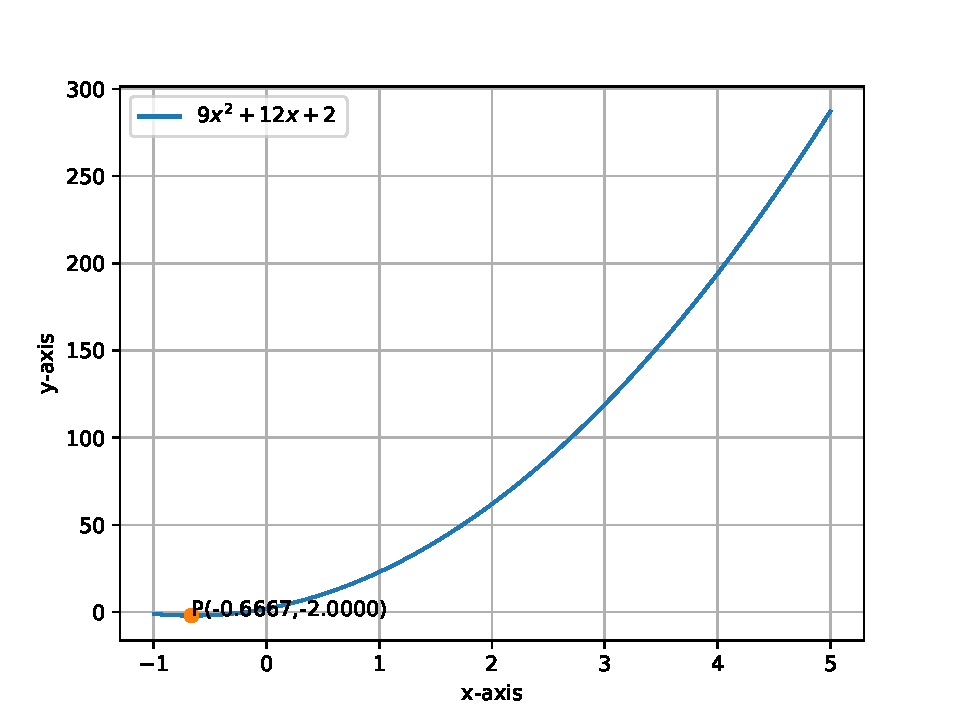
\includegraphics[width=\columnwidth]{12/6/5/1/1/1/figs/opt2.pdf}
	\end{center}
\caption{}
\label{fig:/12/6/5/1/1/convFig1}
\end{figure}

	\end{enumerate}
\item
At what points in the interval (0,2$\pi$) does the function $\sin2x$ attain its maximum value.
\label{12/6/5/8/1}
%\iffalse
\documentclass[journal,10pt,twocolumn]{article}
\usepackage{graphicx, float}
\usepackage[margin=0.5in]{geometry}
\usepackage{amsmath, bm}
\usepackage{array}
\usepackage{booktabs}
\usepackage{mathtools}

\providecommand{\norm}[1]{\left\lVert#1\right\rVert}
\let\vec\mathbf
\newcommand{\myvec}[1]{\ensuremath{\begin{pmatrix}#1\end{pmatrix}}}
\newcommand{\mydet}[1]{\ensuremath{\begin{vmatrix}#1\end{vmatrix}}}

\title{\textbf{Optimization Assignment}}
\author{Maddu Dinesh}
\date{September 2022}

\begin{document}

\maketitle
\paragraph{\textit{Problem Statement} -
\fi
At what points in the interval (0,2$\pi$) does the function $\sin2x$ attain its maximum value.
\\
\solution
	\begin{figure}[!ht]
		\centering
		\includegraphics[width=\columnwidth]{12/6/5/8/figs/a.png}
		\caption{}
		\label{fig:12/6/5/8}
  	\end{figure}
\iffalse
\section*{\large Figure}

\begin{figure}[H]
\centering
\includegraphics[width=1\columnwidth]{a.png}
\caption{Graph of f(x)}
\label{fig:triangle}
\end{figure}
\section*{\large Solution}

	
    \subsection*{\normalsize Gradient descent}
\fi    
  Since  
    \begin{align}
	\label{eq:12/6/5/8vol_varx}
	    f(x) &= \sin2x,
	    \\
	    f'(x) &= 2\cos2x
	\end{align}
\iffalse
we have to attain the maximum value of sin2x in the interval [0,2$\pi$]. This can be seen in Figure f(x).
\fi
Using gradient ascent, 
\begin{align}
	x_{n+1} &= x_n + \alpha \nabla f(x_n) \\
&=x_n+\alpha(2\cos2x)
\end{align}
Choosing
\begin{align}
	x_0&=0.5,\alpha=0.001, precision = 0.00000001, 
	\\
	f_{max} &= 1.0000,
 	x_{max}= 0.7854.
    \end{align}
   
    

    





 







\item
Find the absolute maximum and minimum values of the function $f$ given by 
\begin{align}
	f(x) = \cos^2x + \sin x,\quad x \in \sbrak{0,\pi} 
\end{align} 
\label{12/6/6/14/1}
%\iffalse
\documentclass[10pt,twocolumn]{article}
\usepackage{graphicx}
\usepackage[margin=0.5in]{geometry}
\usepackage[cmex10]{amsmath}
\usepackage{array}
\usepackage{booktabs}
\usepackage{mathtools}
\title{\textbf{Optimization Assignment}}
\author{Sinkona Chinthamalla}

\providecommand{\norm}[1]{\lVert#1\rVert}
\providecommand{\abs}[1]{\vert#1\vert}
\let\vec\mathbf
\newcommand{\myvec}[1]{\ensuremath{\begin{pmatrix}#1\end{pmatrix}}}
\newcommand{\mydet}[1]{\ensuremath{\begin{vmatrix}#1\end{vmatrix}}}
\providecommand{\brak}[1]{\ensuremath{\left(#1\right)}}
\providecommand{\lbrak}[1]{\ensuremath{\left(#1\right.}}
\providecommand{\rbrak}[1]{\ensuremath{\left.#1\right)}}
\providecommand{\sbrak}[1]{\ensuremath{{}\left[#1\right]}}

\begin{document}

\maketitle
\paragraph{\textit{Problem Statement} -
\fi
Find the absolute maximum and minimum values of the function $f$ given by 
\begin{align}
	f(x) = \cos^2x + \sin x,\quad x \in \sbrak{0,\pi} 
\end{align} 
\solution
	\begin{figure}[!ht]
		\centering
		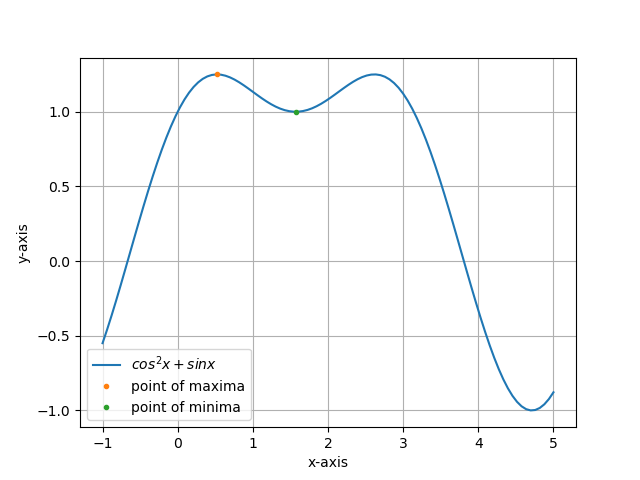
\includegraphics[width=\columnwidth]{12/6/6/14/figs/opt.png}
		\caption{}
		\label{fig:12/6/6/14}
  	\end{figure}
\iffalse

\section{Solution}
\begin{flushleft}
Given function is,\\
\end{flushleft}
\begin{equation}
    f(x)=\cos^2x + \sin x
\end{equation}
\subsection{Calculation using normal differentiation}
\begin{flushleft}
Differentiating (1) yields,
\end{flushleft}
\fi
The derivative of the given function is
\begin{align}
\nabla f(x) = \cos x-2\sin x \cos x 
\end{align}
\iffalse

\noindent Calculating the critical points:
$ \nabla f(x) = 0 $

\begin{equation}
\implies \cos{x} = 0 
\end{equation}
\begin{equation}
\implies -2\sin{x} + 1 = 0
\end{equation}
Therefore, the critical points are 

\begin{equation}
\frac{\pi}{6},\quad\frac{5\pi}{6},\quad\frac{\pi}{2}
\end{equation}

\textbf{1.1.1 Finding absolute maximum and minimum} 
Since given interval is $x \in [0,\pi]$ 

\begin{table}[h]
\centering
\large
\begin{tabular}{|l|l|}
\hline
\textbf{value of x} & \textbf{value of} \\ \hline
At x =0             & 1                 \\ \hline
At x =$ \frac{\pi}{6}$            & $\frac{5}{4}$            \\ \hline
At x =  $ \frac{\pi}{2}$            & 1                 \\ \hline
At x =  $ \frac{5\pi}{6}$            & $\frac{5}{4}$             \\ \hline
at x =       $\pi$       & 1                 \\ \hline
\end{tabular}
\end{table}

Hence, 
\begin{align}
\text{absolute maximum} & =  \frac{5}{4}\\
\text{absolute minimum} & = 1
\end{align}

\subsection{Calculation of Maxima using gradient ascent algorithm}
\fi
The 
maxima is calculated by
\begin{align}
x_{n+1} = x_n + \alpha \nabla f(x_n) 
\\
 &= x_n + \alpha \brak{cosx_n-2sinx_ncosx_n}
\end{align}
where 
\begin{enumerate}
	\item $x_0=0.5$ 
	\item $\alpha=0.001$ 
	\item precision $= 0.00000001$ 
\end{enumerate}
yielding
    \begin{align}
	    f_{max} = 1.25, 
 x_{max}        = 0.52.
    \end{align}
    \iffalse
    
\begin{figure}[h!]
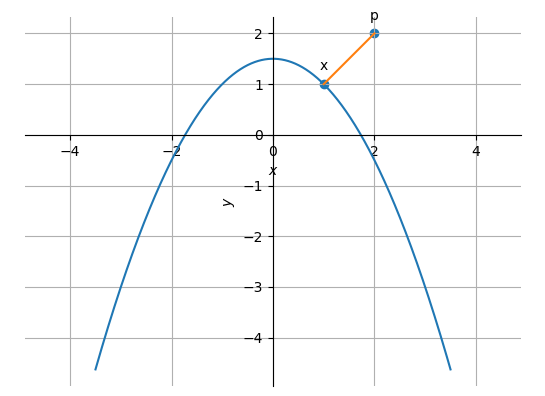
\includegraphics[scale=0.55]{opt.png}
\caption{The function f(x) with maxima and minima points}
\end{figure}        

\subsection{Calculation of Minima using gradient descent algorithm}
To find: 
\begin{align}
\min_{x} f(x)
\end{align}  
Given:
\begin{align}
f(x) = \cos^2x + \sin x,\quad x \in [0,\pi] 
\end{align}
\fi
The 
minima  is found by 
\begin{align}
	x_{n+1} &= x_n - \alpha \nabla f(x_n)
\\
 &= x_n - \alpha \brak{cosx_n-2sinx_ncosx_n}
\end{align}
\iffalse
where \\
1)$x_0=0.5$ \\
2)$\alpha=0.001$ \\
3)precision $= 0.00000001$ \\
values obtained using python are:
    \begin{align}
        \boxed{\text{Minima} = 1 }\\
        \boxed{\text{Minima Point} = 1.57}
    \end{align}

\end{document}
\fi


\end{enumerate}
